\documentclass{ximera}
%%%
\title{TikZ and Tables}
\author{Robert Kelvey, robertkelvey@gmail.com}

\usepackage{multicol}
\usepackage{graphicx}
\usepackage{gnuplottex}
\usepackage[latin1]{inputenc}
\usepackage{tikz}
\usepackage{pgfplots}

\begin{document}

\begin{abstract}
    In this activity, we give drawing a tikZ picture a try and draw some tables.
\end{abstract}

\maketitle

\begin{center}
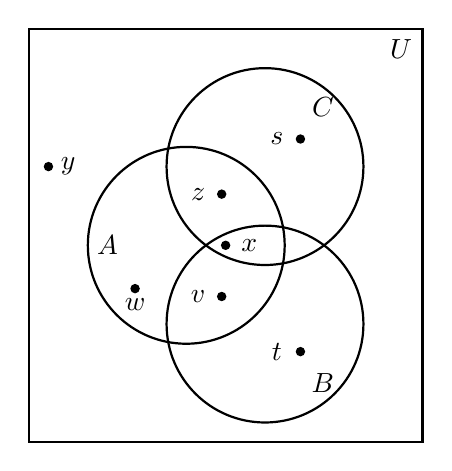
\begin{tikzpicture}
%%%%%DRAW SETS%%%%%%%%%
\draw[thick]  (-2, -2.5) rectangle (3, 2.75) node[below left]{$U$};
\draw[thick] (0,0) circle (1.25cm); 
\draw (-1,0) node {$A$};
\draw[thick] (1,-1) circle (1.25cm); 
\draw (2,-1.75) node[left] {$B$};
\draw[thick] (1,1) circle (1.25cm); 
\draw (2,1.75) node[left] {$C$};

%%%%%DRAW POINTS%%%%%%%
\draw (0.80,0) node {$x$};
\fill[black] (0.50,0) circle (0.06cm); 

\fill[black] (-1.75,1) circle (0.06cm);
\draw (-1.5,1) node {$y$};

\fill[black] (0.45, 0.65) circle (0.06cm);
\draw (0.15,0.65) node {$z$};

\fill[black] (-0.65, -0.55) circle (0.06cm);
\draw (-0.65,-0.75) node {$w$};

\fill[black] (0.45, -0.65) circle (0.06cm);
\draw (0.15,-0.65) node {$v$};

\fill[black] (1.45, -1.35) circle (0.06cm);
\draw (1.15,-1.35) node {$t$};

\fill[black] (1.45, 1.35) circle (0.06cm);
\draw (1.15,1.35) node {$s$};

\end{tikzpicture}
\end{center}

\begin{question}
Identify the following as true or false using the universal set $U$ above and its subsets $A$, $B$, and $C$. \\ Enter your answers with a `T' for true or `F' for false.
    \begin{enumerate}
        \item $v \in A \cap C  \answer[given]{F}$
			
			\item $y \in \bar{A} \cap \bar{B} \cap \bar{C}  \answer{T}$
			
			\item $x \in A - B \answer{F} $
			
			\item $z \in (A \cup C) \cap B  \answer{F}$
			
			\item $\emptyset \subseteq C \answer{T}$
			
			\item $\{w, s, z\} \subseteq (A - C) \cup (C - A) \answer{F}$
			
			\item $\{y,t\} \subseteq \bar{B} \cup \bar{C} \answer{T}$
			
			\item $\{s\} \in \mathcal{P}(C) \answer{T}$
    \end{enumerate}

\end{question}

The above did not use multicols, nor was there a use of the ``prompt" command. We try both below to see what will happen!

\begin{question}
Identify the following as true or false using the universal set $U$ above and its subsets $A$, $B$, and $C$. \\ Enter your answers with a 'T' for true or 'F' for false.
\begin{prompt}
    \begin{enumerate}
    \begin{multicols}{2}

        \item $v \in A \cap C  \answer[given]{F}$
			
			\item $y \in \bar{A} \cap \bar{B} \cap \bar{C}  \answer{T}$
			
			\item $x \in A - B \answer{F} $
			
			\item $z \in (A \cup C) \cap B  \answer{F}$
			
			\item $\emptyset \subseteq C \answer{T}$
			
			\item $\{w, s, z\} \subseteq (A - C) \cup (C - A) \answer{F}$
			
			\item $\{y,t\} \subseteq \bar{B} \cup \bar{C} \answer{T}$
			
			\item $\{s\} \in \mathcal{P}(C) \answer{T}$
    \end{multicols}
    \end{enumerate}
\end{prompt}
\end{question}

In the above, we had the first answer with the ``given" option. Now we list all answers as ``given" in the remixed question below.
\begin{question}
Identify the following as true or false using the universal set $U$ above and its subsets $A$, $B$, and $C$. \\ Enter your answers with a 'T' for true or 'F' for false.
\begin{prompt}
    \begin{enumerate}
    \begin{multicols}{2}

        \item $v \in A \cap C  \answer[given]{F}$
			
			\item $y \in \bar{A} \cap \bar{B} \cap \bar{C}  \answer[given]{T}$
			
			\item $x \in A - B \answer[given]{F} $
			
			\item $z \in (A \cup C) \cap B  \answer[given]{F}$
			
			\item $\emptyset \subseteq C \answer[given]{T}$
			
			\item $\{w, s, z\} \subseteq (A - C) \cup (C - A) \answer[given]{F}$
			
			\item $\{y,t\} \subseteq \bar{B} \cup \bar{C} \answer[given]{T}$
			
			\item $\{s\} \in \mathcal{P}(C) \answer[given]{T}$
    \end{multicols}
    \end{enumerate}
\end{prompt}
\end{question}

Now we try the above but without the single answer prompt. Instead, we employ a multiple choice for each item, with two choices: `T' or `F'.

\begin{question}  
Identify the following as true or false using the universal set $U$ above and its subsets $A$, $B$, and $C$.
\begin{prompt}
\begin{enumerate}
    \begin{multicols}{2}
        \item $v \in A \cap C$
            \begin{multipleChoice}
			    \choice{T}
                \choice[correct]{F}
            \end{multipleChoice} 
			
		\item $y \in \bar{A} \cap \bar{B} \cap \bar{C}$
		    \begin{multipleChoice}
			    \choice[correct]{T}
                \choice{F}
            \end{multipleChoice}	
		\item $x \in A - B$
		    \begin{multipleChoice}
			    \choice{T}
                \choice[correct]{F}
            \end{multipleChoice}	
		\item $z \in (A \cup C) \cap B$
		    \begin{multipleChoice}
			    \choice{T}
                \choice[correct]{F}
            \end{multipleChoice}	
		\item $\emptyset \subseteq C$
		    \begin{multipleChoice}
			    \choice[correct]{T}
                \choice{F}
            \end{multipleChoice}	
		\item $\{w, s, z\} \subseteq (A - C) \cup (C - A)$
		    \begin{multipleChoice}
			    \choice{T}
                \choice[correct]{F}
            \end{multipleChoice}	
		\item $\{y,t\} \subseteq \bar{B} \cup \bar{C}$
		    \begin{multipleChoice}
			    \choice[correct]{T}
                \choice{F}
            \end{multipleChoice}	
		\item $\{s\} \in \mathcal{P}(C)$
	        \begin{multipleChoice}
			    \choice[correct]{T}
                \choice{F}
            \end{multipleChoice}
		\end{multicols} 
\end{enumerate}
\end{prompt}
\end{question}

OKAY so it looks like multiple choice does not like multicols very much (at least in pdf). Let's try that again, but without multicols.

\begin{question}  
Identify the following as true or false using the universal set $U$ above and its subsets $A$, $B$, and $C$.
\begin{prompt}
\begin{enumerate}
        \item $v \in A \cap C$
            \begin{multipleChoice}
			    \choice{T}
                \choice[correct]{F}
            \end{multipleChoice} 
			
		\item $y \in \bar{A} \cap \bar{B} \cap \bar{C}$
		    \begin{multipleChoice}
			    \choice[correct]{T}
                \choice{F}
            \end{multipleChoice}	
		\item $x \in A - B$
		    \begin{multipleChoice}
			    \choice{T}
                \choice[correct]{F}
            \end{multipleChoice}	
		\item $z \in (A \cup C) \cap B$
		    \begin{multipleChoice}
			    \choice{T}
                \choice[correct]{F}
            \end{multipleChoice}	
		\item $\emptyset \subseteq C$
		    \begin{multipleChoice}
			    \choice[correct]{T}
                \choice{F}
            \end{multipleChoice}	
		\item $\{w, s, z\} \subseteq (A - C) \cup (C - A)$
		    \begin{multipleChoice}
			    \choice{T}
                \choice[correct]{F}
            \end{multipleChoice}	
		\item $\{y,t\} \subseteq \bar{B} \cup \bar{C}$
		    \begin{multipleChoice}
			    \choice[correct]{T}
                \choice{F}
            \end{multipleChoice}	
		\item $\{s\} \in \mathcal{P}(C)$
	        \begin{multipleChoice}
			    \choice[correct]{T}
                \choice{F}
            \end{multipleChoice}
\end{enumerate}
\end{prompt}
\end{question}

That seems to look better. 

After publishing this baked xake, can see that the HTML looks terrible. Mainly, multicols does not play nicely in any way.

Our very first question on this activity looks alright. Let us try that again, but place everything into a table to attempt to ``align" various items (like the questions verus the answer boxes).

First, we redraw our TikZ venn diagram (to remind us all about it!). We will try this first without using the enumerate environment. 
\begin{center}
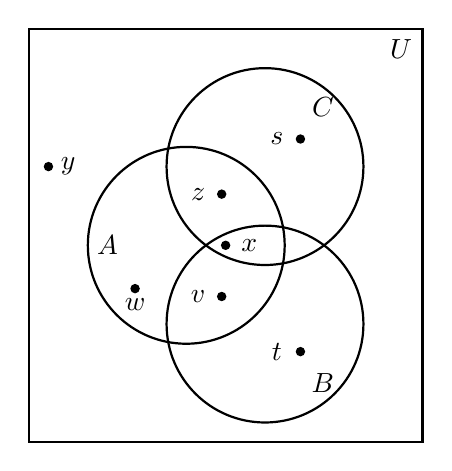
\begin{tikzpicture}
%%%%%DRAW SETS%%%%%%%%%
\draw[thick]  (-2, -2.5) rectangle (3, 2.75) node[below left]{$U$};
\draw[thick] (0,0) circle (1.25cm); 
\draw (-1,0) node {$A$};
\draw[thick] (1,-1) circle (1.25cm); 
\draw (2,-1.75) node[left] {$B$};
\draw[thick] (1,1) circle (1.25cm); 
\draw (2,1.75) node[left] {$C$};

%%%%%DRAW POINTS%%%%%%%
\draw (0.80,0) node {$x$};
\fill[black] (0.50,0) circle (0.06cm); 

\fill[black] (-1.75,1) circle (0.06cm);
\draw (-1.5,1) node {$y$};

\fill[black] (0.45, 0.65) circle (0.06cm);
\draw (0.15,0.65) node {$z$};

\fill[black] (-0.65, -0.55) circle (0.06cm);
\draw (-0.65,-0.75) node {$w$};

\fill[black] (0.45, -0.65) circle (0.06cm);
\draw (0.15,-0.65) node {$v$};

\fill[black] (1.45, -1.35) circle (0.06cm);
\draw (1.15,-1.35) node {$t$};

\fill[black] (1.45, 1.35) circle (0.06cm);
\draw (1.15,1.35) node {$s$};

\end{tikzpicture}
\end{center}

\begin{question}
Identify the following as true or false using the universal set $U$ above and its subsets $A$, $B$, and $C$. \\ Enter your answers with a `T' for true or `F' for false.
\begin{prompt}
\begin{center}
    \begin{tabular}[c]{c c}

$v \in A \cap C$ & $\answer[given]{F}$ \\
			
$y \in \bar{A} \cap \bar{B} \cap \bar{C}$ & $\answer{T}$ \\
			
$x \in A - B$ & $\answer{F} $ \\
			
$z \in (A \cup C) \cap B$ & $\answer{F}$ \\
			
$\emptyset \subseteq C$ & $\answer{T}$\\
			
$\{w, s, z\} \subseteq (A - C) \cup (C - A)$ & $\answer{F}$ \\
$\{y,t\} \subseteq \bar{B} \cup \bar{C}$ & $\answer{T}$ \\
			
$\{s\} \in \mathcal{P}(C)$ & $\answer{T}$ \\
    \end{tabular}
   \end{center}
\end{prompt}
\end{question}

Okay so that looks interesting. What if instead of utilizing the tabular environment, we use the ``align*" environment instead?

\begin{question}
Identify the following as true or false using the universal set $U$ above and its subsets $A$, $B$, and $C$. \\ Enter your answers with a `T' for true or `F' for false.
\begin{prompt}

    \begin{align*}
        v \in A \cap C && \answer[given]{F}  \\
        y \in \bar{A} \cap \bar{B} \cap \bar{C} && \answer{T} \\		
        x \in A - B && \answer{F}  \\		
        z \in (A \cup C) \cap B && \answer{F} \\	
        \emptyset \subseteq C && \answer{T} \\	
        \{w, s, z\} \subseteq (A - C) \cup (C - A) && \answer{F}&\\
        \{y,t\} \subseteq \bar{B} \cup \bar{C} && \answer{T} \\			
        \{s\} \in \mathcal{P}(C) && \answer{T} 
    \end{align*}

\end{prompt}
\end{question}

That looks interesting. Let us try an align tab in the front for some different alignment possibilities?

\begin{question}
Identify the following as true or false using the universal set $U$ above and its subsets $A$, $B$, and $C$. \\ Enter your answers with a `T' for true or `F' for false.
\begin{prompt}

    \begin{align*}
        &v \in A \cap C && \answer[given]{F}  \\
        &y \in \bar{A} \cap \bar{B} \cap \bar{C} && \answer{T} \\		
        &x \in A - B && \answer{F}  \\		
        &z \in (A \cup C) \cap B && \answer{F} \\	
        &\emptyset \subseteq C && \answer{T} \\	
        &\{w, s, z\} \subseteq (A - C) \cup (C - A) && \answer{F}&\\
        &\{y,t\} \subseteq \bar{B} \cup \bar{C} && \answer{T} \\			
        &\{s\} \in \mathcal{P}(C) && \answer{T} 
    \end{align*}

\end{prompt}
\end{question}

Nice! that gave us left-alignment. 

Let us finally try to make a ``fill-in-the-blank" truth table.

\begin{problem}
Fill in the truth table below using your amazing logic skillz!

\begin{prompt}
\begin{center}
\begin{tabular}{c | c | c | c }
		$p$ & $q$ & $p \implies q$ & $p \vee (p \implies q)$ \\
		\hline
		T & T & T & $\answer{T}$ \\
		T & F & F & $\answer{T}$ \\
		F & T & T & $\answer{T}$\\
		F & F & T & $\answer{T}$
	\end{tabular}
\end{center}
\end{prompt}
\end{problem}

Well hey that looks pretty cool. Now we will get a little tricky. Let us try to make a truth table that isn't fill in the blank, but instead gives the options as multiple choice; i.e. a `T' choice and a `F' choice.

\begin{problem}
Fill in the truth table below using your amazing logic skillz!

%\begin{prompt}
%\begin{center}
%\begin{tabular}{c | c | c | c }
%		$p$ & $q$ & $p \implies q$ & $p \vee (p \implies q)$ \\
%		\hline
%		T & T & T & \begin{multipleChoice} \choice[correct]{T} \choice{F} \end{multipleChoice} \\
%		T & F & F & \begin{multipleChoice} \choice[correct]{T} \choice{F} \end{multipleChoice} \\
%		F & T & T & \begin{multipleChoice} \choice[correct]{T} \choice{F} \end{multipleChoice}\\
%		F & F & T & \begin{multipleChoice} \choice[correct]{T} \choice{F} \end{multipleChoice}
%	\end{tabular}
%\end{center}
%\end{prompt}
\end{problem}



\end{document}
